% ============================================================
\chapter{Analyse Spectrale}
\label{ch:spectrale}
% ============================================================

\section{Exemple motivant}
Un signal climatique contient des cycles de diff\'erentes p\'eriodes (journalier, annuel, El Ni\~no). L'analyse spectrale d\'ecompose la variance totale par fr\'equence, r\'ev\'elant les p\'eriodicites cach\'ees.

\section{Densit\'e spectrale}\index{densite spectrale@densit\'e spectrale}

\begin{definition}[Densit\'e spectrale de puissance]
Si $\sum_{h=-\infty}^{\infty}|\gamma(h)|<\infty$, la \textbf{densit\'e spectrale} de $(X_t)$ est :
\[
f(\omega) = \frac{1}{2\pi}\sum_{h=-\infty}^{\infty}\gamma(h)\,e^{-i\omega h}, \quad \omega\in[-\pi,\pi].
\]
C'est la transform\'ee de Fourier de la fonction d'autocovariance.
\end{definition}

\begin{theoreme}[Propri\'et\'es de $f$]
\begin{enumerate}
\item $f(\omega)\geq 0$ pour tout $\omega$.
\item $f$ est paire : $f(\omega)=f(-\omega)$.
\item Relation inverse : $\gamma(h) = \int_{-\pi}^{\pi}f(\omega)\,e^{i\omega h}\,d\omega$.
\item $\gamma(0) = \Var(X_t) = \int_{-\pi}^{\pi}f(\omega)\,d\omega$ (th\'eor\`eme de Parseval).
\end{enumerate}
\end{theoreme}

\begin{proof}[Esquisse de (1)]
Par le th\'eor\`eme de Herglotz, $\gamma$ est semi-d\'efinie positive. Donc $f(\omega)=\frac{1}{2\pi}\sum\gamma(h)e^{-i\omega h}\geq 0$ (comme limite de formes quadratiques positives).
\end{proof}

\section{Spectres de processus classiques}

\begin{theoreme}[Spectre d'un ARMA$(p,q)$]
\[
f(\omega) = \frac{\sigma^2}{2\pi}\,\frac{|\theta(e^{-i\omega})|^2}{|\phi(e^{-i\omega})|^2}.
\]
\end{theoreme}

\begin{exemple}[Spectre d'un AR(1)]
$\phi(z)=1-\phi z$ :
\[
f(\omega) = \frac{\sigma^2}{2\pi}\,\frac{1}{|1-\phi e^{-i\omega}|^2} = \frac{\sigma^2}{2\pi(1-2\phi\cos\omega+\phi^2)}.
\]
Si $\phi>0$ : pic en $\omega=0$ (basses fr\'equences dominantes). Si $\phi<0$ : pic en $\omega=\pi$.
\end{exemple}

\begin{center}
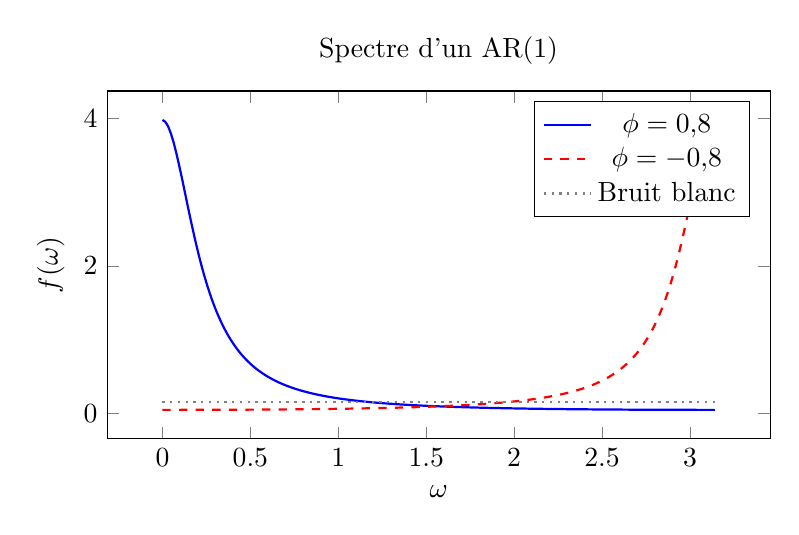
\begin{tikzpicture}
\begin{axis}[
  width=10cm, height=6cm,
  xlabel={$\omega$}, ylabel={$f(\omega)$},
  title={Spectre d'un AR(1)},
  domain=0:3.14159, samples=200,
  legend pos=north east
]
\addplot[thick,blue] {1/(2*3.14159*(1-2*0.8*cos(deg(x))+0.64))};
\addlegendentry{$\phi=0{,}8$}
\addplot[thick,red,dashed] {1/(2*3.14159*(1+2*0.8*cos(deg(x))+0.64))};
\addlegendentry{$\phi=-0{,}8$}
\addplot[thick,gray,dotted] {1/(2*3.14159)};
\addlegendentry{Bruit blanc}
\end{axis}
\end{tikzpicture}
\end{center}

\section{P\'eriodogramme}\index{periodogramme@p\'eriodogramme}

\begin{definition}[P\'eriodogramme]
L'estimateur na\"if de $f(\omega)$ :
\[
I_n(\omega) = \frac{1}{2\pi n}\left|\sum_{t=1}^n X_t\,e^{-i\omega t}\right|^2.
\]
\end{definition}

\begin{theoreme}[Propri\'et\'es du p\'eriodogramme]
\begin{enumerate}
\item $\E[I_n(\omega_j)]\to f(\omega_j)$ pour les fr\'equences de Fourier $\omega_j=2\pi j/n$.
\item $I_n(\omega_j)$ est un estimateur \textbf{non consistant} : $\Var(I_n(\omega_j))\not\to 0$.
\item Aux fr\'equences de Fourier : $I_n(\omega_j)/f(\omega_j)\stackrel{\text{approx}}{\sim}\chi^2(2)/2$.
\end{enumerate}
\end{theoreme}

\begin{attention}
Le p\'eriodogramme brut est tr\`es erratique. Il faut le lisser pour obtenir un estimateur consistant.
\end{attention}

\section{Estimation spectrale}\index{estimation spectrale}

\subsection{Fen\^etre spectrale (lissage)}

\begin{definition}[P\'eriodogramme liss\'e]
\[
\hat{f}(\omega) = \sum_{|h|\leq M} w(h)\,\hat{\gamma}(h)\,e^{-i\omega h},
\]
o\`u $w$ est une \textbf{fen\^etre} (Bartlett, Parzen, Tukey, etc.) et $M$ est la \textbf{largeur de bande}.
\end{definition}

\subsection{M\'ethode param\'etrique}

Estimer un mod\`ele AR$(p)$ par Yule--Walker ou Burg, puis utiliser le spectre th\'eorique $\hat{f}(\omega)=\frac{\hat\sigma^2}{2\pi|\hat\phi(e^{-i\omega})|^2}$.

\section{Impl\'ementation}

\begin{codeblock}[title=\textbf{Python}]
\begin{minted}{python}
import numpy as np
import matplotlib.pyplot as plt
from scipy.signal import periodogram, welch

# Simuler un AR(2) avec pic spectral
np.random.seed(42)
n = 1024
eps = np.random.normal(0, 1, n)
x = np.zeros(n)
phi1, phi2 = 1.5, -0.85  # racines complexes => pic
for t in range(2, n):
    x[t] = phi1*x[t-1] + phi2*x[t-2] + eps[t]

# Périodogramme brut
freq_p, Pxx_p = periodogram(x, fs=1, scaling='density')

# Périodogramme lissé (Welch)
freq_w, Pxx_w = welch(x, fs=1, nperseg=256, scaling='density')

fig, axes = plt.subplots(1, 2, figsize=(14, 5))
axes[0].semilogy(freq_p, Pxx_p, lw=0.5)
axes[0].set_title('Périodogramme brut')
axes[0].set_xlabel('Fréquence')

axes[1].semilogy(freq_w, Pxx_w, lw=1.5, color='red')
axes[1].set_title('Périodogramme lissé (Welch)')
axes[1].set_xlabel('Fréquence')

plt.tight_layout()
plt.savefig('ch07_spectral.pdf')
plt.show()

# Spectre théorique AR(2)
omega = np.linspace(0.01, np.pi, 500)
phi_z = 1 - phi1*np.exp(-1j*omega) - phi2*np.exp(-2j*omega)
f_theo = 1 / (2*np.pi * np.abs(phi_z)**2)

plt.figure(figsize=(8, 4))
plt.plot(omega, f_theo, 'b-', label='Théorique')
plt.title('Spectre théorique AR(2)')
plt.xlabel('$\\omega$'); plt.ylabel('$f(\\omega)$')
plt.legend()
plt.savefig('ch07_spectral_theo.pdf')
plt.show()
\end{minted}
\end{codeblock}

\section{Exercices}

\begin{exercice}[$\star$]
Calculer la densit\'e spectrale d'un MA(1) : $X_t=\eps_t+\theta\eps_{t-1}$.
\end{exercice}

\begin{exercice}[$\star\star$]
Montrer que le p\'eriodogramme peut s'\'ecrire $I_n(\omega)=\sum_{|h|<n}\hat\gamma(h)e^{-i\omega h}/(2\pi)$.
\end{exercice}

\begin{exercice}[$\star\star$]
D\'emontrer que pour un bruit blanc gaussien, $2nI_n(\omega_j)/\sigma^2\sim\chi^2(2)$ aux fr\'equences de Fourier non nulles.
\end{exercice}

\begin{exercice}[$\star\star\star$ -- Projet]
Analyser le spectre des temp\'eratures journali\`eres de Paris sur 50 ans. Identifier les pics correspondant aux cycles annuel, semi-annuel et hebdomadaire.
\end{exercice}

\begin{formules}
\begin{align*}
f(\omega) &= \frac{1}{2\pi}\sum_{h}\gamma(h)e^{-i\omega h}, \quad \gamma(h)=\int_{-\pi}^{\pi}f(\omega)e^{i\omega h}d\omega \\
f_{\text{ARMA}}(\omega) &= \frac{\sigma^2}{2\pi}\frac{|\theta(e^{-i\omega})|^2}{|\phi(e^{-i\omega})|^2} \\
I_n(\omega) &= \frac{1}{2\pi n}\left|\sum_{t=1}^n X_t e^{-i\omega t}\right|^2
\end{align*}
\end{formules}
